\documentclass[a4paper]{report}
\usepackage{hyperref}
\usepackage{lastpage}
\usepackage{fancyhdr}
\usepackage{lineno}
\usepackage{listings}
\usepackage{german}
\usepackage[utf8]{inputenc}
\usepackage{amssymb}
\usepackage{graphicx}
%\newcommand{\genasso}[2]{\begin{minipage}{0.7\textwidth}\begin{normalsize}\begin{flushleft}\textbf{{#1}}\end{flushleft}\end{normalsize}\vspace{-1cm}\begin{flushleft}\begin{small}{#2}\end{small}\end{flushleft}\end{minipage}\\\vspace{0.2cm}}
\pagenumbering{arabic}

\pagestyle{fancy} 
\newcommand{\frontmatter}{\clearpage \cfoot{\thepage\ }
\setcounter{page}{1}
\pagenumbering{Roman}}
\newcommand{\mainmatter}{\clearpage \lhead{\myAuth} \rhead{\myDate} \cfoot{} \rfoot{\thepage\ of \pageref{LastPage}}
\setcounter{page}{1}
\pagenumbering{arabic}}
\newcommand{\backmatter}{\clearpage \rfoot{\thepage\ }
\setcounter{page}{1}
\pagenumbering{alph}}


\newcommand{\makemytitlepage}{\begin{titlepage}
    \begin{center}
        \vspace*{0.8cm}
        
        \Huge
        \textbf{\myTitle}
        
        \vspace{1.5cm}
        
        \Large
        \myAuthor

        \vspace{1.8cm}

        %\begin{large}\textbf{Abstract:} \myAbstract \end{large}
        
\includegraphics[width=6cm]{./IM.jpg}  
        
        \vfill
        
        \huge
        \myAsso
        
        \vspace{1.3cm}
        
        \Large

        %\myDate
        \today
        
    \end{center}
\end{titlepage}}
\newcommand{\myAuth}{Team: *Iron Man*\\B. Pohl, K. Trogant, R. Enseleit, D. Hebecker}
\newcommand{\myAuthor}{Birgit Pohl 574353 (MO. 9-11)\\Kevin Trogant 572451 (Mo. 15-17)\\Ronja Enseleit 572404 (Mo. 15-17)\\Dustin Hebecker 571271 (MO. 9-11)}
\newcommand{\myAsso}{Group: *Iron Man*}
\newcommand{\myDate}{\today}

%%%%%%%%%%%%%%%%%%%%%%%%%%%%%%%%
%%Change Title !!!!!!!!!!!!!!!!!
%%%%%%%%%%%%%%%%%%%%%%%%%%%%%%%%
\newcommand{\myTitle}{Exercise Sheet A}

\begin{document}
\frontmatter
\makemytitlepage
\mainmatter

%%%%%%%%%%%%%%%%%%%%%%%%%%%%%%%%%%%%%%%%%%%%%%%%%%%%%%%%%%
%% Only modify below here and change myTitle!!!!!!!!!!!!!!
%%%%%%%%%%%%%%%%%%%%%%%%%%%%%%%%%%%%%%%%%%%%%%%%%%%%%%%%%%
\section*{Aufgabe 1}
\begin{enumerate}
 \item Project Setup
     \subitem 1.1 Work Packages
     \subitem 1.2 PERT
     \subitem 1.3 Gantt
     \subitem 1.4 Backend Planning
     \subitem 1.6 Backend Setup
     \subitem 1.7 Task Automation Management (Gulp)

\item Features (Stories and Views)
     \subitem 2.1 Order View
    	 \subsubitem 2.1.1 Change Order
    	 \subsubitem 2.1.2 Calculate Distance
        \subsubitem 2.1.3 Calculate Delivery Cost
     \subitem 2.2 Branch View
     	\subsubitem 2.2.1 Authenticate Customer
     	\subsubitem 2.2.2 Block Customer for 30 days
     	\subsubitem 2.2.3 Read, Update Order Status
        \subsubitem 2.2.4 Read, Update Stock per Branch
     \subitem 2.3 Staff View
        \subsubitem 2.3.1 CRUD Recipes
        \subsubitem 2.3.2 Create, Delete Ingredients
     \subitem 2.4 Deliverer View
        \subsubitem 2.4.1 Map
        \subsubitem 2.4.2 Show Delivery address and route        
     \subitem 2.5 Management View  
        \subsubitem 2.5.1 Statistics Receips
        \subsubitem 2.5.2 Statistics Ingredients per Branch
        \subsubitem 2.5.3 PDF Export and download
\end{enumerate}

% Aufgaben:\\
% \begin{itemize}
% \item Erstellung einer Kunden Datenbank\\
% \item Erstellung einer Vorrats-, Fillial-, Rezept und Preis Datenbank\\
% \item Erstellung eines Kunden Web-Interface\\
% \item[-] Subinterface: Bestellung\\
% \item[-] Subinterface: Bestellungsänderungen\\
% \item Erstellung eines Mitarbeiter Interface\\
% \item[-]Subinterface: Bestellungen\\
% \item[-]Subsubinterface: Streckenplanung/Streckenkostenbrechnung\\
% \item[-]Subinterface: Vorräte\\
% \item[-]Subinterface: Rezepte und Preise\\ 
% \item[-]Subaufgabe: PDF export\\
% \end{itemize}
% 
% 
% 
% \ \\Optional:\\
% \begin{itemize}
% \item Verteilung von Lieferungen optimiert nach Bestell-Que und Lieferzeit auf Fillialen verteilen.\\
% \item Konzeptausarbeitung für Pizza-Back-Robot und Dronen-Auslieferung. ;)\\
% \end{itemize}






\newpage
\section*{Aufgabe 2}
        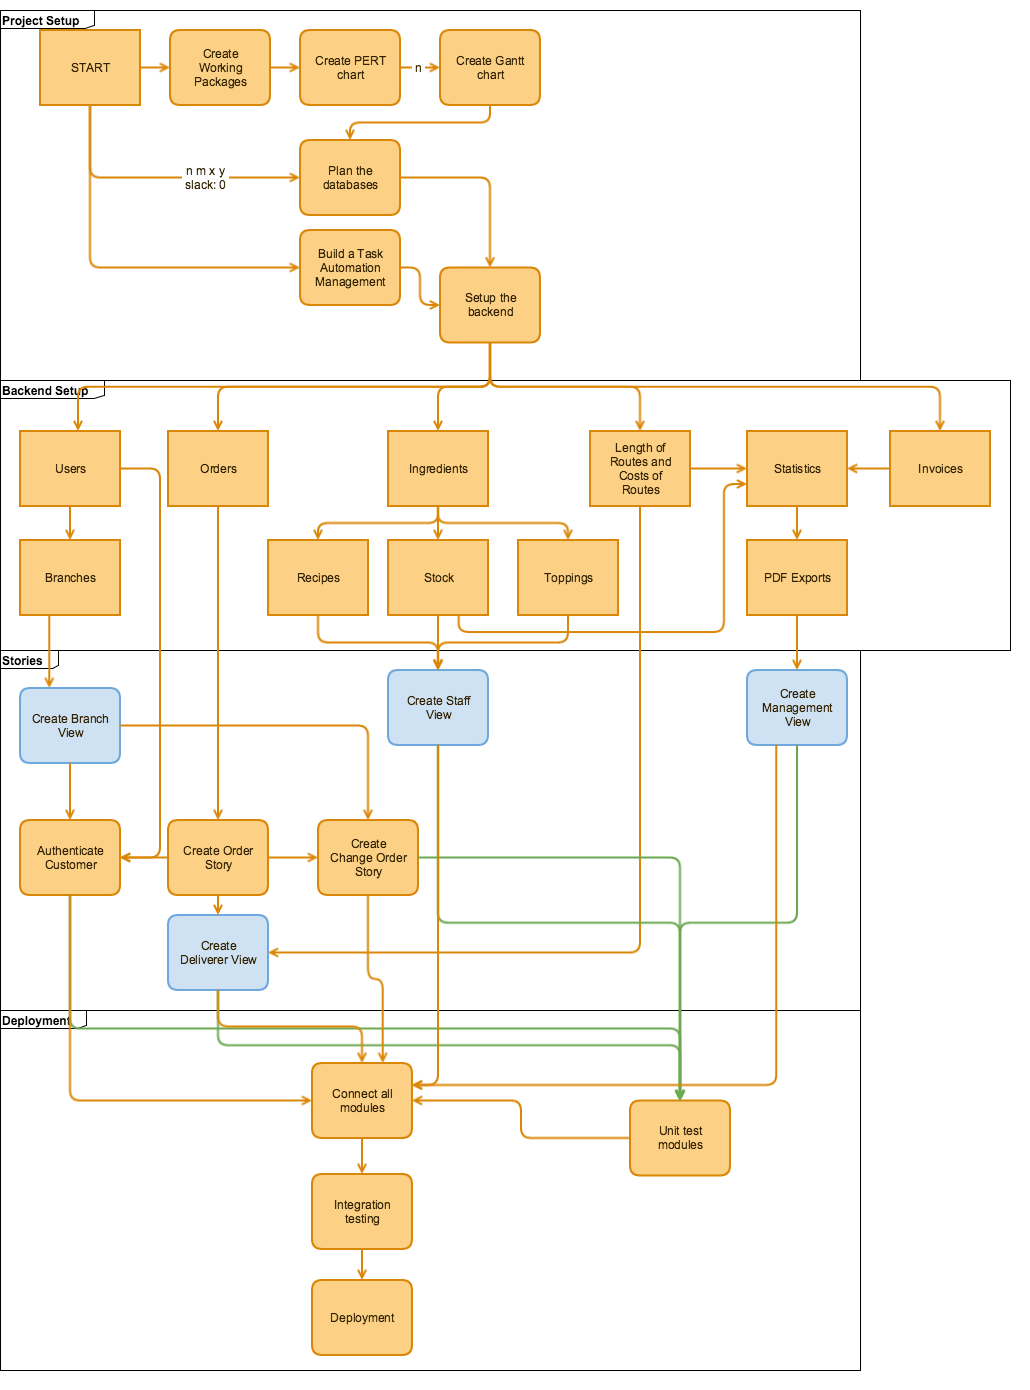
\includegraphics[width=14cm]{./diagramm.png}  

\newpage
\section*{Aufgabe 3}




\end{document}
